\section{Experimental Procedure}

The experiment was initially going to be run on a Linux Laptop, since that was the most convenient to hand, but had to moved to a Windows Desktop machine when a fairly sizable bug was discovered.  It turns out that the icons in the application window do not display correctly when viewed on a lower resolution screen (1366 x 768 in this case) - see figure 1.  This is clearly bad interface design in that the creators of the product did not envisage it to be used on a screen resolution that was smaller than the one they evidently implemented it on.  This flaw makes the system potentially unusable to a number of users, and so if this were a real scenario this bug would need to be corrected before this program were released to the general public.

\begin{figure}[t]
\centering
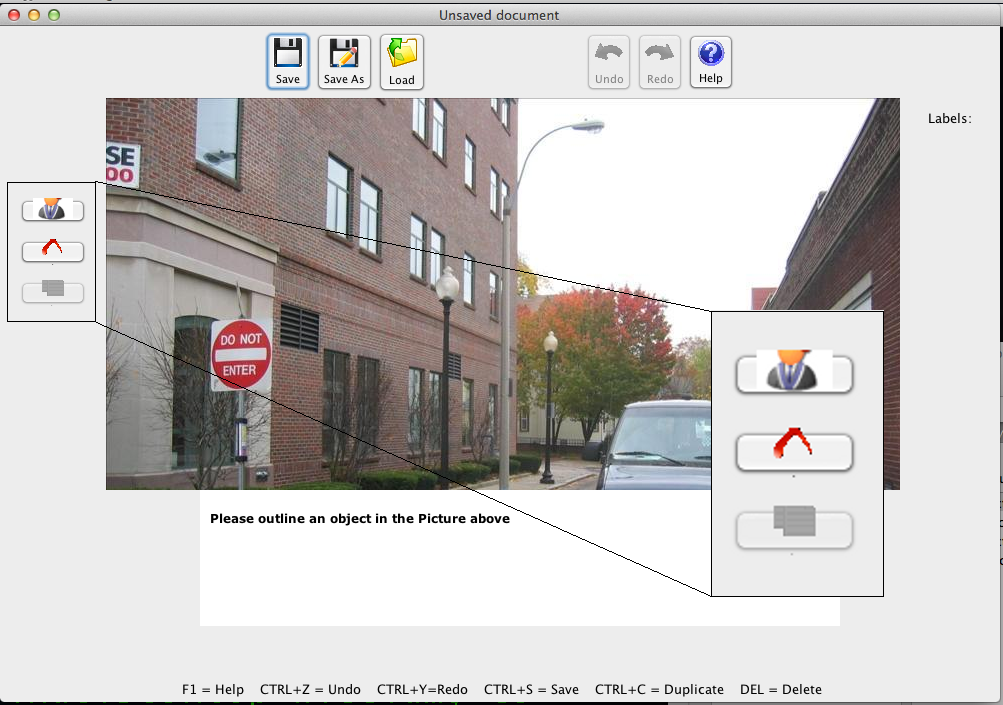
\includegraphics[width=6cm]{sshot2.png}
\caption{A screen-shot of the main window of the application, notice that the zoomed in section has buttons which are squashed causing them to appear to have no label or legible icon}
\label{fig:fullView}
\end{figure}

Having found a monitor that had a large enough resolution display the participant was briefed on what the product was intended to be used for and then asked to give their initial impressions on the interface design.  They were then instructed to carry out several tasks to exercise the full functionality of the program whilst being timed, with the number of mouse clicks required per task also being recorded.  After the successful completion of each operation the thoughts of the participant were taken and they were asked to give a score out of five with regards to how easy they found it to accomplish: one being easy, five being hard.  The tasks were to load an image file, add an annotation, create a second annotation, select an annotation, delete an annotation, edit an annotation, duplicate an annotation, and finally save the annotated image.  This process was repeated three times for an image labelled A, an image labelled B, and finally back to image A.  The purpose of this technique was to observe how the user gained familiarity with the product over time and to ensure they could return to a previously edited file after leaving it.

In the following sections we will discuss what the participant’s thoughts were at each stage of the test and then analyse how those relate to the principles of human-computer interactions.
